\documentclass[aspectratio=169]{beamer}

\makeatletter
\def\input@path{{../BeamerTemplate/theme/}}
\makeatother

\usepackage[utf8]{inputenc}
\usepackage{lmodern}
\usepackage[T1]{fontenc}
\usepackage{listings}
\usepackage{tikz}
\usetikzlibrary{arrows.meta, positioning, shapes.geometric, calc, shapes.multipart, matrix}

\usetheme{CleanEasy}
\input{../BeamerTemplate/configs/configs}

\title{Union-Find (Disjoint Set)}
\subtitle{Data Structures}
\author{Minseok Jeon}
\institute{DGIST}
\date{\today}

\begin{document}

\begin{frame}
  \titlepage
\end{frame}

\begin{frame}{Table of Contents}
  \tableofcontents
\end{frame}

\section{Introduction to Union-Find}

\begin{frame}{What is Union-Find?}
  \textbf{Union-Find (Disjoint Set)} is a data structure that maintains dynamic connectivity across disjoint sets.

  \vspace{0.5cm}
  \textbf{Key Concepts:}
  \begin{itemize}
    \item \textbf{Disjoint Set:} Collection of non-overlapping sets
    \item \textbf{Representative:} Each set has a representative (root) element
    \item \textbf{Parent Array:} Each element points to its parent
    \item \textbf{Forest:} Multiple trees, each representing a set
  \end{itemize}

  \vspace{0.5cm}
  \textbf{Core Operations:}
  \begin{itemize}
    \item \texttt{find(x)}: Find the representative of x's set
    \item \texttt{union(x, y)}: Merge the sets containing x and y
    \item \texttt{connected(x, y)}: Check if x and y are in the same set
  \end{itemize}
\end{frame}

\begin{frame}{Visual Representation}
  \textbf{Initial State (n=5):}
  \begin{center}
    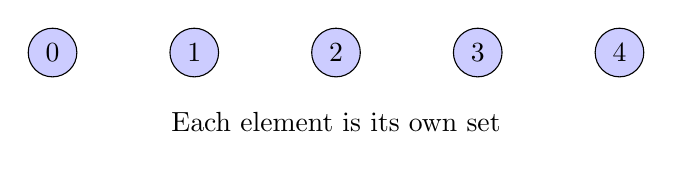
\begin{tikzpicture}[scale=0.9]
      \foreach \i in {0,1,2,3,4} {
        \node[circle, draw, fill=blue!20] (n\i) at (\i*2,0) {\i};
      }
      \node[below] at (4,-0.7) {Each element is its own set};
    \end{tikzpicture}
  \end{center}

  \vspace{0.5cm}
  \textbf{After union(0,1) and union(2,3):}
  \begin{center}
    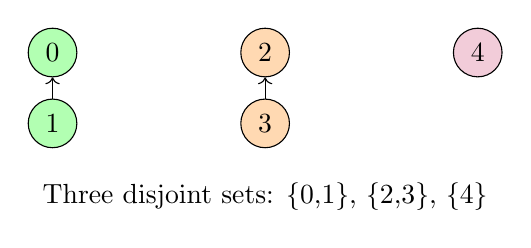
\begin{tikzpicture}[scale=0.9]
      % First tree: 0-1
      \node[circle, draw, fill=green!30] (n0) at (0,0) {0};
      \node[circle, draw, fill=green!30] (n1) at (0,-1) {1};
      \draw[->] (n1) -- (n0);

      % Second tree: 2-3
      \node[circle, draw, fill=orange!30] (n2) at (3,0) {2};
      \node[circle, draw, fill=orange!30] (n3) at (3,-1) {3};
      \draw[->] (n3) -- (n2);

      % Third tree: 4
      \node[circle, draw, fill=purple!20] (n4) at (6,0) {4};

      \node[below] at (3,-1.7) {Three disjoint sets: \{0,1\}, \{2,3\}, \{4\}};
    \end{tikzpicture}
  \end{center}
\end{frame}

\begin{frame}{Applications}
  Union-Find has numerous practical applications:

  \vspace{0.3cm}
  \begin{enumerate}
    \item \textbf{Kruskal's Algorithm:} Finding minimum spanning trees
    \item \textbf{Network Connectivity:} Checking if nodes can communicate
    \item \textbf{Percolation:} Modeling fluid flow through materials
    \item \textbf{Image Segmentation:} Grouping similar pixels
    \item \textbf{Social Networks:} Finding friend circles
    \item \textbf{Cycle Detection:} Detecting cycles in undirected graphs
    \item \textbf{Dynamic Equivalence:} Tracking equivalent elements
    \item \textbf{Number of Islands:} Counting connected components in a grid
  \end{enumerate}

  \vspace{0.3cm}
  \textbf{Key Advantage:} Nearly O(1) operations with proper optimizations!
\end{frame}

\section{Basic Implementation}

\begin{frame}[fragile]{Naive Implementation}
  \begin{lstlisting}[language=Python, basicstyle=\ttfamily\footnotesize]
class UnionFind:
    def __init__(self, n):
        # Initially, each element is its own parent
        self.parent = list(range(n))
        self.count = n  # Number of disjoint sets

    def find(self, x):
        """Find root of element x"""
        while self.parent[x] != x:
            x = self.parent[x]
        return x

    def union(self, x, y):
        """Merge sets containing x and y"""
        root_x = self.find(x)
        root_y = self.find(y)

        if root_x != root_y:
            self.parent[root_x] = root_y
            self.count -= 1

    def connected(self, x, y):
        """Check if x and y are in same set"""
        return self.find(x) == self.find(y)
  \end{lstlisting}
\end{frame}

\begin{frame}[fragile]{Example Usage}
  \begin{lstlisting}[language=Python, basicstyle=\ttfamily\footnotesize]
# Create Union-Find with 5 elements
uf = UnionFind(5)

# Union operations
uf.union(0, 1)  # Merge {0} and {1}
uf.union(2, 3)  # Merge {2} and {3}
uf.union(0, 2)  # Merge {0,1} and {2,3}

# Check connectivity
print(uf.connected(1, 3))  # True (both in {0,1,2,3})
print(uf.connected(1, 4))  # False (4 is separate)
print(uf.count)            # 2 sets: {0,1,2,3}, {4}
  \end{lstlisting}

  \vspace{0.5cm}
  \textbf{Problem:} This naive implementation can be slow!
  \begin{itemize}
    \item Worst case: Linear chain of elements
    \item \texttt{find} operation: O(n) time
    \item \texttt{union} operation: O(n) time
  \end{itemize}
\end{frame}

\begin{frame}{Problem: Linear Chains}
  \textbf{Worst Case Scenario:}

  \begin{center}
    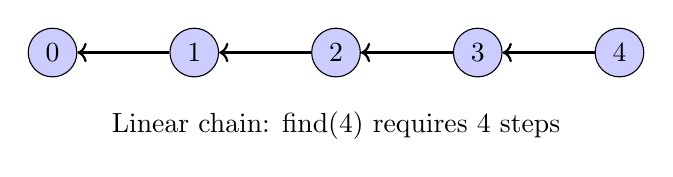
\begin{tikzpicture}[scale=0.9]
      \node[circle, draw, fill=blue!20] (n0) at (0,0) {0};
      \node[circle, draw, fill=blue!20] (n1) at (2,0) {1};
      \node[circle, draw, fill=blue!20] (n2) at (4,0) {2};
      \node[circle, draw, fill=blue!20] (n3) at (6,0) {3};
      \node[circle, draw, fill=blue!20] (n4) at (8,0) {4};

      \draw[->, thick] (n1) -- (n0);
      \draw[->, thick] (n2) -- (n1);
      \draw[->, thick] (n3) -- (n2);
      \draw[->, thick] (n4) -- (n3);

      \node[below] at (4,-0.7) {Linear chain: find(4) requires 4 steps};
    \end{tikzpicture}
  \end{center}

  \vspace{0.5cm}
  \textbf{Consequences:}
  \begin{itemize}
    \item Sequential unions can create long chains
    \item Each \texttt{find} operation walks entire chain
    \item Multiple finds: O(n) each time
    \item Overall complexity: O(n) per operation
  \end{itemize}

  \vspace{0.3cm}
  \textbf{Solution:} We need optimizations!
\end{frame}

\section{Path Compression}

\begin{frame}{Path Compression Idea}
  \textbf{Optimization 1: Path Compression}

  \vspace{0.3cm}
  \textbf{Key Insight:}
  \begin{itemize}
    \item During \texttt{find}, we walk from x to root
    \item Why not make every node on path point directly to root?
    \item Future \texttt{find} operations become faster!
  \end{itemize}

  \vspace{0.5cm}
  \textbf{Before find(4):}
  \begin{center}
    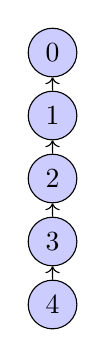
\begin{tikzpicture}[scale=0.8]
      \node[circle, draw, fill=blue!20] (n0) at (2,0) {0};
      \node[circle, draw, fill=blue!20] (n1) at (2,-1) {1};
      \node[circle, draw, fill=blue!20] (n2) at (2,-2) {2};
      \node[circle, draw, fill=blue!20] (n3) at (2,-3) {3};
      \node[circle, draw, fill=blue!20] (n4) at (2,-4) {4};

      \draw[->] (n1) -- (n0);
      \draw[->] (n2) -- (n1);
      \draw[->] (n3) -- (n2);
      \draw[->] (n4) -- (n3);
    \end{tikzpicture}
  \end{center}
\end{frame}

\begin{frame}{Path Compression Effect}
  \textbf{After find(4) with path compression:}

  \begin{center}
    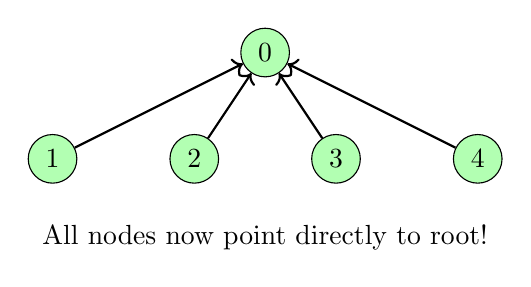
\begin{tikzpicture}[scale=0.9]
      \node[circle, draw, fill=green!30] (n0) at (4,0) {0};
      \node[circle, draw, fill=green!30] (n1) at (1,-1.5) {1};
      \node[circle, draw, fill=green!30] (n2) at (3,-1.5) {2};
      \node[circle, draw, fill=green!30] (n3) at (5,-1.5) {3};
      \node[circle, draw, fill=green!30] (n4) at (7,-1.5) {4};

      \draw[->, thick] (n1) -- (n0);
      \draw[->, thick] (n2) -- (n0);
      \draw[->, thick] (n3) -- (n0);
      \draw[->, thick] (n4) -- (n0);

      \node[below] at (4,-2.3) {All nodes now point directly to root!};
    \end{tikzpicture}
  \end{center}

  \vspace{0.5cm}
  \textbf{Benefits:}
  \begin{itemize}
    \item Tree becomes flatter
    \item Future \texttt{find} operations: O(1)
    \item Amortized complexity improves significantly
  \end{itemize}
\end{frame}

\begin{frame}[fragile]{Path Compression Implementation}
  \textbf{Recursive Implementation:}
  \begin{lstlisting}[language=Python, basicstyle=\ttfamily\footnotesize]
def find(self, x):
    """Find with path compression"""
    if self.parent[x] != x:
        # Recursively find root and compress path
        self.parent[x] = self.find(self.parent[x])
    return self.parent[x]
  \end{lstlisting}

  \vspace{0.5cm}
  \textbf{Iterative Implementation:}
  \begin{lstlisting}[language=Python, basicstyle=\ttfamily\footnotesize]
def find_iterative(self, x):
    """Iterative find with path compression"""
    root = x
    # Find root
    while self.parent[root] != root:
        root = self.parent[root]

    # Compress path: point all nodes to root
    while x != root:
        next_parent = self.parent[x]
        self.parent[x] = root
        x = next_parent

    return root
  \end{lstlisting}
\end{frame}

\begin{frame}[fragile]{Path Halving Optimization}
  \textbf{Path Halving:} Point every other node to its grandparent (one-pass)

  \begin{lstlisting}[language=Python, basicstyle=\ttfamily\footnotesize]
def find_path_halving(self, x):
    """Point every other node to its grandparent"""
    while self.parent[x] != x:
        self.parent[x] = self.parent[self.parent[x]]
        x = self.parent[x]
    return x
  \end{lstlisting}

  \vspace{0.5cm}
  \textbf{Advantages:}
  \begin{itemize}
    \item Single pass (no recursion or two passes)
    \item Simpler and more efficient
    \item Still achieves excellent amortized complexity
    \item Popular in competitive programming
  \end{itemize}
\end{frame}

\section{Union by Rank}

\begin{frame}{Union by Rank Idea}
  \textbf{Optimization 2: Union by Rank}

  \vspace{0.3cm}
  \textbf{Problem with Naive Union:}
  \begin{itemize}
    \item Always attach first tree to second
    \item Can create unbalanced trees
    \item Results in long chains
  \end{itemize}

  \vspace{0.5cm}
  \textbf{Solution: Union by Rank}
  \begin{itemize}
    \item \textbf{Rank:} Upper bound on tree height
    \item \textbf{Rule:} Attach smaller rank tree under larger rank tree
    \item \textbf{Benefit:} Keeps trees balanced
    \item Trees grow logarithmically
  \end{itemize}

  \vspace{0.5cm}
  \textbf{Rank Update Rules:}
  \begin{itemize}
    \item If ranks differ: Attach smaller under larger, no rank change
    \item If ranks equal: Attach either way, increase winner's rank by 1
  \end{itemize}
\end{frame}

\begin{frame}{Union by Rank Example}
  \textbf{Tree A (rank 1):}
  \begin{center}
    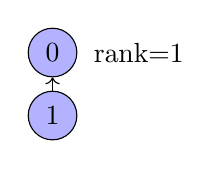
\begin{tikzpicture}[scale=0.8]
      \node[circle, draw, fill=blue!30] (n0) at (0,0) {0};
      \node[circle, draw, fill=blue!30] (n1) at (0,-1) {1};
      \draw[->] (n1) -- (n0);
      \node[right] at (0.5,0) {rank=1};
    \end{tikzpicture}
  \end{center}

  \vspace{0.3cm}
  \textbf{Tree B (rank 2):}
  \begin{center}
    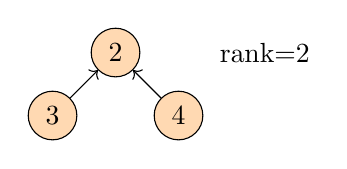
\begin{tikzpicture}[scale=0.8]
      \node[circle, draw, fill=orange!30] (n2) at (2,0) {2};
      \node[circle, draw, fill=orange!30] (n3) at (1,-1) {3};
      \node[circle, draw, fill=orange!30] (n4) at (3,-1) {4};
      \draw[->] (n3) -- (n2);
      \draw[->] (n4) -- (n2);
      \node[right] at (3.5,0) {rank=2};
    \end{tikzpicture}
  \end{center}

  \vspace{0.3cm}
  \textbf{After union(0, 2): Attach A under B (smaller rank under larger)}
  \begin{center}
    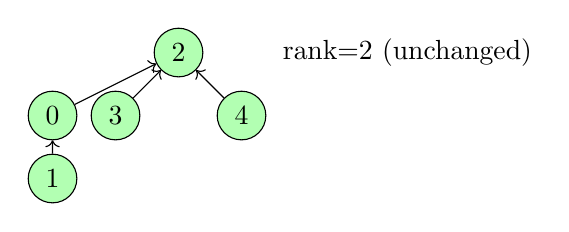
\begin{tikzpicture}[scale=0.8]
      \node[circle, draw, fill=green!30] (n2) at (3,0) {2};
      \node[circle, draw, fill=green!30] (n3) at (2,-1) {3};
      \node[circle, draw, fill=green!30] (n4) at (4,-1) {4};
      \node[circle, draw, fill=green!30] (n0) at (1,-1) {0};
      \node[circle, draw, fill=green!30] (n1) at (1,-2) {1};

      \draw[->] (n3) -- (n2);
      \draw[->] (n4) -- (n2);
      \draw[->] (n0) -- (n2);
      \draw[->] (n1) -- (n0);

      \node[right] at (4.5,0) {rank=2 (unchanged)};
    \end{tikzpicture}
  \end{center}
\end{frame}

\begin{frame}[fragile]{Union by Rank Implementation}
  \begin{lstlisting}[language=Python, basicstyle=\ttfamily\footnotesize]
class UnionFindRank:
    def __init__(self, n):
        self.parent = list(range(n))
        self.rank = [0] * n  # Initial rank is 0
        self.count = n

    def find(self, x):
        if self.parent[x] != x:
            self.parent[x] = self.find(self.parent[x])
        return self.parent[x]

    def union(self, x, y):
        root_x = self.find(x)
        root_y = self.find(y)

        if root_x == root_y:
            return False

        # Attach smaller rank tree under larger rank tree
        if self.rank[root_x] < self.rank[root_y]:
            self.parent[root_x] = root_y
        elif self.rank[root_x] > self.rank[root_y]:
            self.parent[root_y] = root_x
        else:
            # Equal rank: attach either way, increase rank
            self.parent[root_y] = root_x
            self.rank[root_x] += 1

        self.count -= 1
        return True
  \end{lstlisting}
\end{frame}

\section{Union by Size}

\begin{frame}{Union by Size}
  \textbf{Alternative: Union by Size}

  \vspace{0.3cm}
  \textbf{Idea:}
  \begin{itemize}
    \item Track number of elements in each tree
    \item Attach smaller tree under larger tree
    \item Also keeps trees balanced
  \end{itemize}

  \vspace{0.5cm}
  \textbf{Comparison with Union by Rank:}
  \begin{itemize}
    \item \textbf{Rank:} Upper bound on height (less accurate with path compression)
    \item \textbf{Size:} Exact count of elements (always accurate)
    \item Both achieve O($\alpha$(n)) complexity with path compression
    \item Size is more intuitive and provides useful information
  \end{itemize}

  \vspace{0.5cm}
  \textbf{Additional Benefits of Size:}
  \begin{itemize}
    \item Can query component size: \texttt{get\_size(x)}
    \item Track largest component: \texttt{max\_size}
    \item Useful for many applications
  \end{itemize}
\end{frame}

\begin{frame}[fragile]{Union by Size Implementation}
  \begin{lstlisting}[language=Python, basicstyle=\ttfamily\footnotesize]
class UnionFindSize:
    def __init__(self, n):
        self.parent = list(range(n))
        self.size = [1] * n  # Initial size is 1
        self.count = n

    def find(self, x):
        if self.parent[x] != x:
            self.parent[x] = self.find(self.parent[x])
        return self.parent[x]

    def union(self, x, y):
        root_x = self.find(x)
        root_y = self.find(y)

        if root_x == root_y:
            return False

        # Attach smaller tree under larger tree
        if self.size[root_x] < self.size[root_y]:
            self.parent[root_x] = root_y
            self.size[root_y] += self.size[root_x]
        else:
            self.parent[root_y] = root_x
            self.size[root_x] += self.size[root_y]

        self.count -= 1
        return True

    def get_size(self, x):
        """Get size of set containing x"""
        return self.size[self.find(x)]
  \end{lstlisting}
\end{frame}

\section{Complexity Analysis}

\begin{frame}[fragile]{The Ackermann Function}
  \textbf{Ackermann Function A(m, n):} Grows extremely fast

  \vspace{0.3cm}
  \begin{lstlisting}[language=Python, basicstyle=\ttfamily\footnotesize]
def A(m, n):
    if m == 0:
        return n + 1
    if n == 0:
        return A(m - 1, 1)
    return A(m - 1, A(m, n - 1))
  \end{lstlisting}

  \vspace{0.3cm}
  \textbf{Growth Rate:}
  \begin{itemize}
    \item A(0, n) = n + 1
    \item A(1, n) = n + 2
    \item A(2, n) = 2n + 3
    \item A(3, n) = $2^{n+3}$ - 3
    \item A(4, n) = $2^{2^{2^{...}}}$ (n+3 times) - 3
  \end{itemize}

  \vspace{0.3cm}
  A(4, 2) is already larger than the number of atoms in the universe!
\end{frame}

\begin{frame}{Inverse Ackermann Function}
  \textbf{Inverse Ackermann $\alpha$(n):} Grows extremely slowly

  \vspace{0.3cm}
  $\alpha$(n) = minimum m such that A(m, m) $\geq$ n

  \vspace{0.5cm}
  \textbf{Values of $\alpha$(n):}
  \begin{itemize}
    \item $\alpha$(1) = 1
    \item $\alpha$(3) = 2
    \item $\alpha$(7) = 3
    \item $\alpha$(2047) = 4
    \item $\alpha$($2^{2048}$ - 1) = 5
  \end{itemize}

  \vspace{0.5cm}
  \textbf{Practical Implication:}
  \begin{itemize}
    \item For all practical n (even n = $10^{80}$), $\alpha$(n) $\leq$ 5
    \item Effectively constant time!
    \item For n = $10^9$, $\alpha$(n) $\approx$ 4
  \end{itemize}
\end{frame}

\begin{frame}{Complexity Comparison}
  \begin{table}
    \centering
    \begin{tabular}{|l|c|c|c|c|}
      \hline
      \textbf{Operation} & \textbf{Naive} & \textbf{Path Comp} & \textbf{Union Rank} & \textbf{Both} \\
      \hline
      Find & O(n) & O(log n)* & O(log n) & O($\alpha$(n))* \\
      \hline
      Union & O(n) & O(log n)* & O(log n) & O($\alpha$(n))* \\
      \hline
      Connected & O(n) & O(log n)* & O(log n) & O($\alpha$(n))* \\
      \hline
      Space & O(n) & O(n) & O(n) & O(n) \\
      \hline
    \end{tabular}
  \end{table}

  \vspace{0.3cm}
  * Amortized complexity

  \vspace{0.5cm}
  \textbf{Key Insights:}
  \begin{itemize}
    \item Path compression alone: O(log n) amortized
    \item Union by rank alone: O(log n) worst case
    \item Both together: O($\alpha$(n)) amortized $\approx$ O(1)
    \item Space is always O(n)
  \end{itemize}
\end{frame}

\begin{frame}{Practical Performance}
  \textbf{Example: $10^9$ operations on $10^9$ elements}

  \vspace{0.5cm}
  \begin{table}
    \centering
    \begin{tabular}{|l|r|r|}
      \hline
      \textbf{Implementation} & \textbf{Complexity} & \textbf{Operations} \\
      \hline
      Naive & O(n) & $10^{18}$ \\
      \hline
      Path Compression & O(log n) & $\sim$ $3 \times 10^{10}$ \\
      \hline
      Union by Rank & O(log n) & $\sim$ $3 \times 10^{10}$ \\
      \hline
      Both Optimized & O($\alpha$(n)) & $\sim$ $4 \times 10^9$ \\
      \hline
    \end{tabular}
  \end{table}

  \vspace{0.5cm}
  \textbf{Speedup with both optimizations:}
  \begin{itemize}
    \item vs Naive: $\sim$ 250 million times faster!
    \item vs Single optimization: $\sim$ 7.5 times faster
    \item Practically constant time per operation
  \end{itemize}
\end{frame}

\section{Applications}

\begin{frame}[fragile]{Kruskal's Minimum Spanning Tree}
  \textbf{Problem:} Find minimum spanning tree of weighted graph

  \begin{lstlisting}[language=Python, basicstyle=\ttfamily\footnotesize]
def kruskal_mst(n, edges):
    """
    Find MST using Kruskal's algorithm
    n: number of vertices
    edges: list of (weight, u, v)
    """
    # Sort edges by weight
    edges.sort()

    uf = UnionFind(n)
    mst = []
    total_weight = 0

    for weight, u, v in edges:
        # If u and v not connected, add edge
        if uf.union(u, v):
            mst.append((u, v, weight))
            total_weight += weight

            # MST complete when n-1 edges added
            if len(mst) == n - 1:
                break

    return mst, total_weight
  \end{lstlisting}

  \textbf{Time Complexity:} O(E log E) for sorting + O(E $\alpha$(V)) for Union-Find
\end{frame}

\begin{frame}[fragile]{Network Connectivity}
  \begin{lstlisting}[language=Python, basicstyle=\ttfamily\footnotesize]
class NetworkConnectivity:
    """Check if network is fully connected"""
    def __init__(self, n):
        self.uf = UnionFind(n)

    def add_connection(self, u, v):
        """Add connection between nodes u and v"""
        self.uf.union(u, v)

    def is_connected(self, u, v):
        """Check if u and v can communicate"""
        return self.uf.connected(u, v)

    def is_fully_connected(self):
        """Check if all nodes are connected"""
        return self.uf.count == 1

    def count_components(self):
        """Count number of separate networks"""
        return self.uf.count

# Example usage
network = NetworkConnectivity(5)
network.add_connection(0, 1)
network.add_connection(2, 3)
print(network.count_components())  # 3: {0,1}, {2,3}, {4}
print(network.is_fully_connected())  # False
  \end{lstlisting}
\end{frame}

\begin{frame}[fragile]{Number of Islands}
  \textbf{Problem:} Count islands in 2D grid ('1' = land, '0' = water)

  \begin{lstlisting}[language=Python, basicstyle=\ttfamily\footnotesize]
def num_islands(grid):
    """Count islands in 2D grid"""
    if not grid:
        return 0

    rows, cols = len(grid), len(grid[0])
    uf = UnionFind(rows * cols)

    def get_id(r, c):
        return r * cols + c

    # Union adjacent land cells
    for r in range(rows):
        for c in range(cols):
            if grid[r][c] == '1':
                # Check right neighbor
                if c + 1 < cols and grid[r][c + 1] == '1':
                    uf.union(get_id(r, c), get_id(r, c + 1))

                # Check down neighbor
                if r + 1 < rows and grid[r + 1][c] == '1':
                    uf.union(get_id(r, c), get_id(r + 1, c))

    # Count unique roots for land cells
    islands = set()
    for r in range(rows):
        for c in range(cols):
            if grid[r][c] == '1':
                islands.add(uf.find(get_id(r, c)))

    return len(islands)
  \end{lstlisting}
\end{frame}

\begin{frame}[fragile]{Cycle Detection}
  \textbf{Problem:} Detect cycle in undirected graph

  \begin{lstlisting}[language=Python, basicstyle=\ttfamily\footnotesize]
def has_cycle(n, edges):
    """Check if undirected graph has cycle"""
    uf = UnionFind(n)

    for u, v in edges:
        # If u and v already connected, adding edge creates cycle
        if uf.connected(u, v):
            return True
        uf.union(u, v)

    return False

# Example: Triangle graph
edges = [(0, 1), (1, 2), (2, 0)]
print(has_cycle(3, edges))  # True
  \end{lstlisting}

  \vspace{0.5cm}
  \textbf{Why it works:}
  \begin{itemize}
    \item In a tree with n nodes: exactly n-1 edges, no cycles
    \item Adding edge between already-connected nodes creates cycle
    \item Union-Find efficiently detects this condition
  \end{itemize}
\end{frame}

\begin{frame}[fragile]{Friend Circles}
  \textbf{Problem:} Count number of friend circles (transitive friendships)

  \begin{lstlisting}[language=Python, basicstyle=\ttfamily\footnotesize]
def find_circle_num(is_connected):
    """
    Count number of friend circles
    is_connected[i][j] = 1 if person i and j are friends
    """
    n = len(is_connected)
    uf = UnionFind(n)

    for i in range(n):
        for j in range(i + 1, n):
            if is_connected[i][j] == 1:
                uf.union(i, j)

    return uf.count

# Example
is_connected = [
    [1, 1, 0],  # Person 0 friends with 0,1
    [1, 1, 0],  # Person 1 friends with 0,1
    [0, 0, 1]   # Person 2 friends with only 2
]
print(find_circle_num(is_connected))  # 2 circles: {0,1}, {2}
  \end{lstlisting}

  \textbf{Key Insight:} Friendship is transitive - if A-B and B-C are friends, then A and C are in same circle
\end{frame}

\begin{frame}[fragile]{Redundant Connection}
  \textbf{Problem:} Find edge that creates cycle in tree

  \begin{lstlisting}[language=Python, basicstyle=\ttfamily\footnotesize]
def find_redundant_connection(edges):
    """Find edge that creates cycle in tree"""
    n = len(edges)
    uf = UnionFind(n + 1)

    for u, v in edges:
        if not uf.union(u, v):
            # Union failed: u and v already connected
            # This edge creates a cycle
            return [u, v]

    return []

# Example: Tree edges with one extra
edges = [[1,2], [1,3], [2,3]]
print(find_redundant_connection(edges))  # [2,3]
  \end{lstlisting}

  \vspace{0.3cm}
  \textbf{Explanation:}
  \begin{itemize}
    \item Process edges in order
    \item First two edges: 1-2, 1-3 form valid tree
    \item Third edge 2-3: nodes already connected via 1, creates cycle
  \end{itemize}
\end{frame}

\section{Advanced Patterns}

\begin{frame}[fragile]{Complete Optimized Implementation}
  \begin{lstlisting}[language=Python, basicstyle=\ttfamily\footnotesize]
class UnionFind:
    """Union-Find with all optimizations"""
    def __init__(self, n):
        self.parent = list(range(n))
        self.rank = [0] * n
        self.count = n

    def find(self, x):
        """Find with path compression"""
        if self.parent[x] != x:
            self.parent[x] = self.find(self.parent[x])
        return self.parent[x]

    def union(self, x, y):
        """Union by rank"""
        root_x = self.find(x)
        root_y = self.find(y)

        if root_x == root_y:
            return False

        if self.rank[root_x] < self.rank[root_y]:
            self.parent[root_x] = root_y
        elif self.rank[root_x] > self.rank[root_y]:
            self.parent[root_y] = root_x
        else:
            self.parent[root_y] = root_x
            self.rank[root_x] += 1

        self.count -= 1
        return True
  \end{lstlisting}
\end{frame}

\begin{frame}[fragile]{Union-Find with Size Tracking}
  \begin{lstlisting}[language=Python, basicstyle=\ttfamily\footnotesize]
class UnionFindWithSize:
    """Track size of each component"""
    def __init__(self, n):
        self.parent = list(range(n))
        self.size = [1] * n
        self.count = n
        self.max_size = 1  # Track largest component

    def union(self, x, y):
        root_x = self.find(x)
        root_y = self.find(y)

        if root_x == root_y:
            return False

        # Always attach smaller to larger
        if self.size[root_x] < self.size[root_y]:
            self.parent[root_x] = root_y
            self.size[root_y] += self.size[root_x]
            self.max_size = max(self.max_size, self.size[root_y])
        else:
            self.parent[root_y] = root_x
            self.size[root_x] += self.size[root_y]
            self.max_size = max(self.max_size, self.size[root_x])

        self.count -= 1
        return True

    def get_size(self, x):
        """Get size of component containing x"""
        return self.size[self.find(x)]
  \end{lstlisting}
\end{frame}

\begin{frame}[fragile]{Union-Find with Custom Data}
  \begin{lstlisting}[language=Python, basicstyle=\ttfamily\footnotesize]
class UnionFindCustom:
    """Union-Find with custom merge function"""
    def __init__(self, n, merge_fn=None):
        self.parent = list(range(n))
        self.rank = [0] * n
        self.data = [None] * n  # Store custom data
        self.merge_fn = merge_fn or (lambda a, b: a)
        self.count = n

    def set_data(self, x, data):
        """Set data for element x"""
        self.data[x] = data

    def get_data(self, x):
        """Get data for component containing x"""
        return self.data[self.find(x)]

    def union(self, x, y):
        root_x = self.find(x)
        root_y = self.find(y)

        if root_x == root_y:
            return False

        # Merge data using custom function
        merged_data = self.merge_fn(self.data[root_x],
                                     self.data[root_y])
        # ... attach trees and store merged_data ...
  \end{lstlisting}
\end{frame}

\begin{frame}[fragile]{Example: Component Sum Tracking}
  \begin{lstlisting}[language=Python, basicstyle=\ttfamily\footnotesize]
# Create Union-Find that tracks sum of each component
uf = UnionFindCustom(5, merge_fn=lambda a, b: a + b)

# Initialize with values 0, 1, 2, 3, 4
for i in range(5):
    uf.set_data(i, i)

# Merge components
uf.union(0, 1)  # Component sum: 0+1 = 1
uf.union(2, 3)  # Component sum: 2+3 = 5

print(uf.get_data(0))  # 1 (sum of component {0,1})
print(uf.get_data(2))  # 5 (sum of component {2,3})
print(uf.get_data(4))  # 4 (sum of component {4})

uf.union(0, 2)  # Merge: 1+5 = 6
print(uf.get_data(0))  # 6 (sum of component {0,1,2,3})
  \end{lstlisting}

  \vspace{0.3cm}
  \textbf{Use Cases:}
  \begin{itemize}
    \item Track minimum/maximum in component
    \item Count properties across component
    \item Accumulate weights or costs
  \end{itemize}
\end{frame}

\section{Summary}

\begin{frame}{Summary: Union-Find Structure}
  \textbf{Core Data Structure:}
  \begin{itemize}
    \item Parent array representing forest of trees
    \item Each tree is a disjoint set
    \item Root of tree is representative of set
  \end{itemize}

  \vspace{0.5cm}
  \textbf{Core Operations:}
  \begin{itemize}
    \item \texttt{find(x)}: Find representative of x's set
    \item \texttt{union(x, y)}: Merge sets containing x and y
    \item \texttt{connected(x, y)}: Check if x and y in same set
  \end{itemize}

  \vspace{0.5cm}
  \textbf{Key Optimizations:}
  \begin{itemize}
    \item \textbf{Path Compression:} Flatten trees during find
    \item \textbf{Union by Rank/Size:} Keep trees balanced
    \item \textbf{Together:} Nearly O(1) operations!
  \end{itemize}
\end{frame}

\begin{frame}{Summary: Complexity}
  \begin{table}
    \centering
    \begin{tabular}{|l|c|c|}
      \hline
      \textbf{Configuration} & \textbf{Time per Op} & \textbf{Space} \\
      \hline
      Naive & O(n) & O(n) \\
      \hline
      Path Compression only & O(log n)* & O(n) \\
      \hline
      Union by Rank only & O(log n) & O(n) \\
      \hline
      Both Optimizations & O($\alpha$(n))* $\approx$ O(1) & O(n) \\
      \hline
    \end{tabular}
  \end{table}

  \vspace{0.3cm}
  * Amortized complexity

  \vspace{0.5cm}
  \textbf{Practical Performance:}
  \begin{itemize}
    \item $\alpha$(n) $\leq$ 5 for all practical n
    \item Essentially constant time operations
    \item Linear space overhead
    \item Extremely efficient in practice
  \end{itemize}
\end{frame}

\begin{frame}{Summary: Applications}
  \textbf{Common Applications:}
  \begin{enumerate}
    \item Kruskal's MST algorithm
    \item Network connectivity problems
    \item Percolation theory
    \item Image processing / segmentation
    \item Dynamic graph connectivity
    \item Cycle detection in graphs
    \item Finding connected components
    \item Social network analysis
  \end{enumerate}

  \vspace{0.5cm}
  \textbf{When to Use Union-Find:}
  \begin{itemize}
    \item Need to group elements into disjoint sets
    \item Frequent connectivity queries
    \item Dynamic merging of groups
    \item Offline processing of relationships
  \end{itemize}
\end{frame}

\begin{frame}{Key Takeaways}
  \begin{enumerate}
    \item Union-Find efficiently maintains disjoint sets
    \item Simple parent array representation
    \item Two key optimizations:
      \begin{itemize}
        \item Path compression (flatten on find)
        \item Union by rank/size (balance trees)
      \end{itemize}
    \item Together achieve O($\alpha$(n)) $\approx$ O(1) per operation
    \item Extremely practical and widely applicable
    \item Easy to implement, hard to beat performance
    \item Essential for graph algorithms (Kruskal's)
    \item Versatile for connectivity problems
  \end{enumerate}

  \vspace{0.5cm}
  \textbf{Remember:} Always use both optimizations in practice!
\end{frame}

\begin{frame}{Practice Problems}
  \textbf{LeetCode Problems:}
  \begin{itemize}
    \item 200. Number of Islands
    \item 547. Number of Provinces (Friend Circles)
    \item 684. Redundant Connection
    \item 685. Redundant Connection II
    \item 721. Accounts Merge
    \item 990. Satisfiability of Equality Equations
    \item 1319. Number of Operations to Make Network Connected
    \item 1579. Remove Max Number of Edges to Keep Graph Traversable
  \end{itemize}

  \vspace{0.5cm}
  \textbf{Advanced:}
  \begin{itemize}
    \item Minimum Spanning Tree problems
    \item Dynamic connectivity with deletions
    \item Persistent Union-Find
  \end{itemize}
\end{frame}

\begin{frame}{Further Learning}
  \textbf{Topics to Explore:}
  \begin{itemize}
    \item Persistent Union-Find (immutable/versioned)
    \item Union-Find with rollback
    \item Weighted Union-Find (for shortest paths)
    \item Link-Cut Trees (more powerful, more complex)
    \item Applications in competitive programming
  \end{itemize}

  \vspace{0.5cm}
  \textbf{Resources:}
  \begin{itemize}
    \item "Introduction to Algorithms" (CLRS) - Chapter 21
    \item "Algorithms" by Sedgewick \& Wayne - Chapter 1.5
    \item Tarjan's original papers on Union-Find analysis
    \item Competitive programming books (Halim, etc.)
  \end{itemize}
\end{frame}

\begin{frame}
  \begin{center}
    {\Huge Thank You!}

    \vspace{1cm}
    {\Large Questions?}

    \vspace{1cm}
    \textit{Union-Find: Simple, Elegant, Efficient}
  \end{center}
\end{frame}

\end{document}
